\chapter{Fejlesztői dokumentáció} % Developer guide
\label{ch:impl}

Ez a fejezet fejlesztőknek nyújt segítséget a ScrumHelper feltérképezésében. Az alfejezetek kifejtik az alkalmazás felépítését, részletesen leírják a különböző rétegeinek (Adatbázis-Szerver-Nézet) osztályait és függvényeit. A vizuális segítséghez különböző diagrammokat is tartalmaz (osztály-, csomag-, felhasználói esetek diagram). A fejezet végén egy tesztforgatókönyv ad részletes leírást a teszt esetek és azok eredményeiről.

\section{Konfiguráció}
\label{config}

A futtatáshoz szükséges előkövetelmények a felhasználói dokumentáció \ref{install}. alfejezetében olvashatók. A dolgozatt keretein belül csak a lokális szerveren való konfigurálás és futtatás lesz részletezve. A különböző szervergépeken való futtatáshoz részletesebb információt a hivatalos Django dokumentációban lehet találni. Utóbbi eset külön konfigurációt igényel a wsgi.py, illetve asgi.py file-ok és környezeti változók megfelelő beállításának segítségével \footnote{wsgi szerver: \url{https://docs.djangoproject.com/en/3.0/howto/deployment/wsgi/} asgi szerver: \url{https://docs.djangoproject.com/en/3.0/howto/deployment/asgi/}}.  

Ahhoz, hogy lokálisan futtatni tudjuk a szervert, először is a ScrumHelper/ScrumHelper/setting.py file-ban kell beállítanunk a DATABSES változót. A pontos beállításai eltérőek a különböző adatbázisok esetében, ehhez részletes segítséget nyújt a hivatalos Django dokumentáció. Alább  egy PostgreSQL adatbázis konfigurációja látható:

\lstset{caption={Konfiguráció PostgreSQL adatbázis használatához}, label=src:settingsconf}
\begin{lstlisting}[language={python}]

DATABASES = {
    'default': {
        'ENGINE': 'django.db.backends.postgresql',
        'NAME': 'database name',
        'USER': 'database user',
        'PASSWORD': 'password',
        'HOST': '127.0.0.1',
        'PORT': '5432',
    }
}

\end{lstlisting}

Ha ez megfelelően van beállítva, akkor a ScrumHelper fő mappába navigálva kell lefuttatni a" python manage.py migrate" parancsot minden első futtatásnál a szükséges adatbázis struktúra kialakításához(illetve ha fejlesztés során olyasmi változik, amely érinti az adatbázis struktúrát, akkor a makemigrations-t is le kell a migrate parancs előtt futtatni). Ezután a "python manage.py runserver" elindítja a lokális szervert a localhost:8000-es portján. Superuser-t, azaz minden jogosultsággal rendelkező felhasználót a szerver futtatása nélkül lehet generálni: "python manage.py createsuperuser" paranccsal, megadva a felhasználónevet és jelszavat utána.

A TIMEZONE változóban adható meg az időzóna. Az egyes projektekhez feltöltött fájlokat a MEDIA\_ROOT konfigurációs változóbeli elérési úton elhelyezkedő mappába menti (ez alapból a ScrumHelper/media könyvtárra mutat). Ugyanezen az elven kezeli a statikus fájlokat is a keretrendszer, ennek a környezeti változója a STATIC\_ROOT.

Fontos, hogy mielőtt az alkalmazás valós, produkciós használatba kerülne szükséges a DEBUG változót False, azaz hamisra állítani (biztonásgi okokból).

\section{Funkcionális terv}

Az \ref{fig:usecase}. ábrán egy felhasználói eset diagram mutatja be az alkalmazás funkcióit:

\begin{figure}[H]
	\centering
	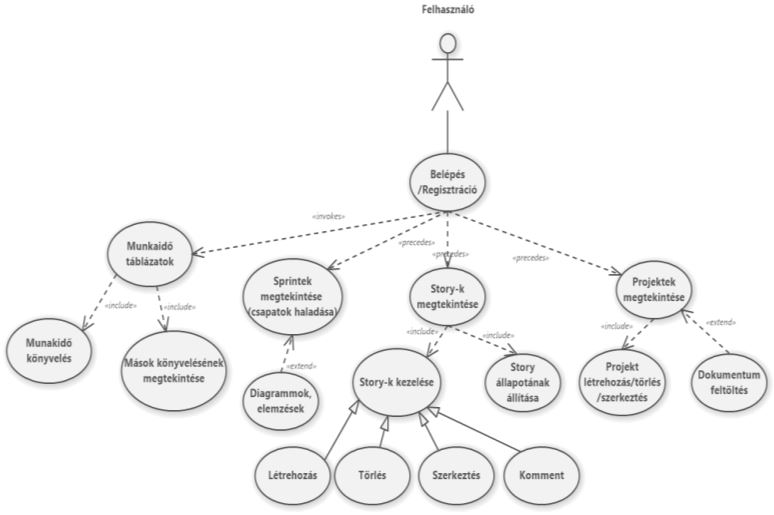
\includegraphics[width=1\textwidth,height=300px]{usecase}
	\caption{Felhasználói eset diagram}
	\label{fig:usecase}
\end{figure}

\section{Struktúrális felépítés}

A ScrumHelper egy MVC (Model-View-Controller) alkalmazás, bár a hivatalos Django dokumentációban az MTV (Model-Template-View) kifejezést használják, mivel ezt gondolják pontosabb leírásának. Tekintve, hogy Djangoban írodott az alkalamzás, ezért ebben a dokumentációban is utóbbi analógia a mérvadó. Ez azt jelenti, hogy három rétegből tevődik össze: egy Model rétegből, amely az adatbázist hivatott reprezentálni, egy View rétegből, amely az adatot reprezentálja (ez alatt azt értjük, amit az adatbázisből kigyűjtött, nem feltétlenül a felhasználó számára megjelnített adatot), valamint a különböző template-ek renderelését is végzi, továbbá egy Template rétegből, mely leírja, hogyan legyen az adat megjelenítve a felhasználó számára.

\begin{figure}[H]
	\centering
	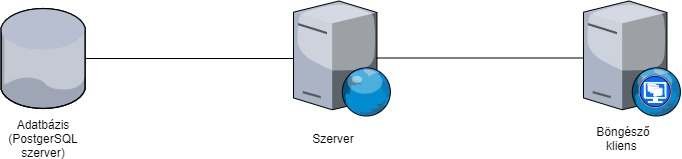
\includegraphics[width=1\textwidth,height=125px]{architecture}
	\caption{Az alkalamzás rétegei: egy adatbázis, egy szerver, ami kinyeri belőle az adatot és továbbítja a nézetnek, valamint a nézet amit a böngészőben láthatunk.}
	\label{fig:architecture}
\end{figure}

